% CVPR 2023 Paper Template
% based on the CVPR template provided by Ming-Ming Cheng (https://github.com/MCG-NKU/CVPR_Template)
% modified and extended by Stefan Roth (stefan.roth@NOSPAMtu-darmstadt.de)

\documentclass[10pt,twocolumn,letterpaper]{article}

%%%%%%%%% PAPER TYPE  - PLEASE UPDATE FOR FINAL VERSION
% \usepackage[review]{cvpr}      % To produce the REVIEW version
\usepackage{cvpr}              % To produce the CAMERA-READY version
%\usepackage[pagenumbers]{cvpr} % To force page numbers, e.g. for an arXiv version

% Include other packages here, before hyperref.
\usepackage{graphicx}
\usepackage{booktabs}
\usepackage{wrapfig}
\usepackage{lipsum}
\usepackage{cite}
\usepackage{amsmath,amssymb,amsfonts}
% \usepackage{textcomp}
% \usepackage{subfloat}
% \usepackage{xcolor}
% \usepackage{wasysym}
% \usepackage{hyperref}
% \usepackage{amsthm}
% \usepackage{mathrsfs}
% \usepackage{txfonts}
% \usepackage{stfloats}
% \usepackage{cite}
% \usepackage{cases}
% %\usepackage{subfig}
% \usepackage{xtab}
% \usepackage{longtable}
% \usepackage{multirow}
% \usepackage{algorithm}
% \usepackage{algpseudocode}
% \usepackage{enumerate}
% \usepackage{enumitem}
% \usepackage{mathtools}
% \usepackage{multicol}
% \usepackage{multirow}
% \usepackage{diagbox}
% \usepackage{amsthm}
% \usepackage{float}
% \usepackage{comment}
% \usepackage{caption}
% \usepackage{subcaption}
% \usepackage[english]{babel}
% \usepackage{url}
% \usepackage{authblk}


% It is strongly recommended to use hyperref, especially for the review version.
% hyperref with option pagebackref eases the reviewers' job.
% Please disable hyperref *only* if you encounter grave issues, e.g. with the
% file validation for the camera-ready version.
%
% If you comment hyperref and then uncomment it, you should delete
% ReviewTempalte.aux before re-running LaTeX.
% (Or just hit 'q' on the first LaTeX run, let it finish, and you
%  should be clear).
\usepackage[pagebackref,breaklinks,colorlinks]{hyperref}


% Support for easy cross-referencing
\usepackage[capitalize]{cleveref}
\crefname{section}{Sec.}{Secs.}
\Crefname{section}{Section}{Sections}
\Crefname{table}{Table}{Tables}
\crefname{table}{Tab.}{Tabs.}


%%%%%%%%% PAPER ID  - PLEASE UPDATE
\def\cvprPaperID{*****} % *** Enter the CVPR Paper ID here
\def\confName{CVPR}
\def\confYear{2023}


\begin{document}

%%%%%%%%% TITLE - PLEASE UPDATE
\title{Super-Resolution for Enhancing Classification Accuracy on Medical Images}

% Use one of these two author templates. Either works
% The first is a custom template, and not the actual CVPR one
\author{Aditya Somasundaram \qquad Sumanth N R \qquad Ruthwika Boyapally \qquad Gautham Bellamkonda\\
\textit{Indian Institute of Technology Hyderabad, India}\\
{\tt\small \{ee20btech11002, ma20btech11016, ma20btech11004, cs20btech11017\}@iith.ac.in}
}

% \author{Aditya Somasundaram\\
% {\tt\small ee20btech11002}
% \and
% Sumanth N R\\
% {\tt\small ma20btech11016}
% \and
% Ruthwika Boyapally\\
% {\tt\small ma20btech11004}
% \and
% Gautham Bellamkonda\\
% {\tt\small cs20btech11017}
% }
\maketitle

%%%%%%%%% ABSTRACT
\begin{abstract}
   Super-Resolution (SR) techniques have shown promise in enhancing the spatial quality and detail of medical images, addressing issues arising from various imaging constraints, such as limited equipment capabilities, low radiation doses, compressed data transmission, and constrained imaging time. However, its potential impact on the overall quality of medical image analysis and diagnosis remains largely unexplored. We aim to explore how SR affects the identification of critical diagnostic features, with a particular emphasis on its potential to enhance classification accuracy in medical image analysis.
\end{abstract}

%%%%%%%%% BODY TEXT
\section{Introduction}
\label{sec:intro}

Super-Resolution (SR) refers to the process of enhancing the resolution or level of detail in an image or video beyond its original resolution. This technique is widely used in various fields, including image processing, computer vision, and medical imaging. There are two primary approaches to super-resolution.

\subsection{Single-Image Super-Resolution (SISR)} In SISR, the goal is to increase the resolution of a single low-resolution image. This is a challenging task as the missing high-frequency details need to be inferred. Deep learning techniques, particularly Convolutional Neural Networks (CNNs), have shown remarkable success in SISR. These networks are trained on pairs of low and high-resolution images to learn the mapping function that can upscale the low-resolution image to a higher resolution while preserving or generating fine details.

\subsection{Multi-Image Super-Resolution (MISR)}
In MISR, multiple low-resolution images of the same scene are used to generate a high-resolution output. This approach takes advantage of the redundancy of information present in multiple images of the same scene, typically captured from slightly different perspectives or with small shifts. Techniques like image registration and fusion are employed to combine these images into a single, high-resolution result.

\subsection{Applications}
\begin{enumerate}
    \item Image and Video Enhancement: Super-resolution can improve the visual quality of images and videos, making them clearer and more detailed.
    \item Medical Imaging: In medical imaging, super-resolution can be used to enhance the quality of MRI or CT scans, enabling better diagnosis and treatment planning.
    \item Surveillance and Security: It can help in improving the quality of surveillance camera footage, making it easier to identify individuals and objects.
    \item Satellite and Remote Sensing: Super-resolution is used to enhance the resolution of satellite images, aiding in various applications such as land-use classification and environmental monitoring.
    \item Art Restoration: Super-resolution techniques can be applied to restore and enhance old or damaged artworks and historical documents.
\end{enumerate}

The effectiveness of super-resolution techniques often depends on the quality of the algorithms and the amount of training data available. Deep learning methods, especially Generative Adversarial Networks (GANs), have made significant strides in achieving impressive super-resolution results by learning complex patterns and structures from large datasets. As technology continues to advance, super-resolution techniques are likely to become even more powerful and applicable in various domains.

%-------------------------------------------------------------------------
\section{Problem Statement}
\label{sec:problem}

Super-Resolution (SR) techniques have shown promise in enhancing the spatial quality and detail of medical images, addressing issues arising from various imaging constraints, such as limited equipment capabilities, low radiation doses, compressed data transmission, and constrained imaging time. However, while SR can significantly improve image resolution, its potential impact on the overall quality of medical image analysis and diagnosis remains largely unexplored.

Current approaches primarily focus on the application of SR to medical images with the objective of improving visual clarity and detail. Nevertheless, there exists a critical knowledge gap regarding how SR impacts the diagnostic accuracy and clinical utility of these enhanced medical images. Specifically, it is unclear how SR affects the identification of critical diagnostic features, the reliability of automated image analysis algorithms.

Therefore, there is an imperative need to investigate the broader implications of SR in the context of medical image analysis beyond mere visual enhancement. We aim to comprehensively examine the effects of SR on the accuracy, reliability, and clinical relevance of medical image analysis. Specifically, we aim to investigate whether SR can be used to enhance discriminative diagnostic features, such that the transformed images are more amenable to classification. By addressing this gap, we seek to unlock the full potential of SR techniques in the field of medical imaging, ultimately advancing patient care, diagnosis, and treatment planning.

% Accurate classification of medical images is of paramount importance in modern healthcare, as it directly impacts diagnostic precision, treatment planning, and patient outcomes. However, a persistent challenge in this domain is the accurate classification of low-resolution medical images, which are often encountered due to various imaging constraints, such as limited equipment capabilities, low radiation doses, constrained imaging time, or compressed data transmission.

% Low-resolution medical images inherently suffer from a deficiency in spatial detail and clarity, creating a obstacle for automated classification algorithms in their task of identifying crucial diagnostic features. Consequently, this limitation can lead to misclassifications, potentially compromising patient care and clinical decision-making.


\section{Literature Review}
Dong et al. \cite{dong2015image} were pioneers in utilizing deep learning methods to address super-resolution challenges in the context of natural image datasets. Building on this foundation, Kim et al. \cite{kim2016accurate} introduced very deep convolutional networks to achieve even more accurate image super-resolution. Following this, Lim et al. \cite{lim2017enhanced} extended the application of deep learning with enhanced deep residual networks, emphasizing the role of residual learning in capturing fine image details. Meanwhile, Kim et al. \cite{kim2016deeply} explored the concept of deeply-recursive convolutional networks, incorporating multiple recursive stages within a CNN to progressively enhance image resolution. Further advancements came with Tai et al. \cite{tai2017image} introducing deep recursive residual networks tailored for image super-resolution, providing an innovative approach to reconstructing high-resolution details. Shifting focus to generative adversarial networks (GANs), Ledig et al. \cite{ledig2017photo} presented a GAN-based approach for photo-realistic single image super-resolution, highlighting the potential of GANs in generating high-quality images. In the realm of GANs, Wang et al. \cite{wang2018esrgan} proposed enhanced Super-Resolution Generative Adversarial Networks (ESRGAN), emphasizing the application of GANs for improved super-resolution quality. 

Shifting toward medical image analysis, Mahaprata et al. \cite{mahapatra2019image} \cite{mahapatra2017retinal} applied progressive GANs to enhance the resolution of medical images, expanding the utility of GANs to healthcare contexts and also combined super-resolution with retinal vasculature segmentation using GANs, demonstrating the applicability of GANs in medical image enhancement. In the field of medical diagnostics, Umehara et al. \cite{umehara2018application} applied super-resolution convolutional neural networks to improve image resolution in chest CT scans. Furthermore, Park et al. \cite{park2018computed} explored the use of deep convolutional neural networks to enhance the resolution of computed tomography (CT) images, offering potential benefits for medical diagnostics. Recent advancements include a Nature Scientific Reports article by Ahmad et al. \cite{ahmad_nature} introducing a novel GAN architecture specifically designed for medical image super-resolution, representing cutting-edge developments in the field. 

Collectively, these papers reflect the diverse approaches and methodologies employed in image super-resolution, from deep learning and recursive architectures to the application of GANs, with significant implications for various domains, including healthcare and diagnostics.

\textbf{Very Low Resolution Image Classification}\cite{vest2017very} utilizes a super resolution net to improve the image resolution before passing it through a network. Comparision of Low Resolution (LR), High Resolution (HR) and Super Resolution (SR) show that the HR gives the best accuracy. closely followed by SRResNet \cite{ledig2017photo} SR Classifier which beats the bicubic interpolation considerably.

% We aim to do the same but on the datasets pertaining to medical images.

\section{Our Methodology}
We aim to study how enhancing the resolution of medical images helps in improving classification accuracy. 
The resolution of the images is increased using two methods: bicubic interpolation and the SRResNet \cite{ledig2017photo}. Convolutional Neural Networks are trained on the two generated datasets and the results are compared. 

Bicubic interpolation is an image resizing technique that estimates pixel values at non-integer coordinates based on neighboring pixels. It employs a smooth cubic function to perform weighted averaging of 16 nearby pixels, resulting in high-quality and visually smooth resized images. However, it's not a learned model like neural networks but rather a deterministic mathematical operation.

\subsection{Architecture of the SRResNet}
The SRResNet \cite{ledig2017photo} architecture is essentially a generator network designed for super-resolution tasks, and it leverages residual blocks to improve image quality and resolution. We employed 16 residual blocks to enhance the quality and resolution of the super-resolved images. This approach is different from traditional super-resolution methods that minimize pixel-wise errors like Mean Squared Error (MSE).

\subsubsection{Residual Blocks:}
This is a building block for the residual network.The block is designed to help the network capture residual information, which is the difference between the super-resolved image and the low-resolution input image. This allows for easier training and the generation of high-quality results.Each Residual Block consists of the following key elements:
\begin{enumerate}
    \item Convolutional Layers: There are two convolutional layers within each Residual Block. These layers have 64 output channels, utilize 3x3 kernels, and are responsible for convolving the input features to extract relevant information.
    \item Instance Normalization: Instance normalization is applied to normalize the features within the Residual Block, aiding in faster convergence and improved training stability.
    \item LeakyReLU Activation: A LeakyReLU activation function is employed with a slope of 0.2. LeakyReLU introduces non-linearity, allowing the network to learn complex mappings, and mitigating the vanishing gradient problem.
\end{enumerate}

\subsubsection{Generator Network:}
\begin{enumerate}
    \item Residual Blocks: The core of the Generator Network consists of 16 Residual Blocks, each comprising two 3x3 convolutional layers with 64 feature maps, batch normalization for enhanced training stability, and LeakyReLU activation functions for introducing non-linearity.

    \item Convolutional Layers: The network commences with a convolutional layer that processes the input image, transforming it into a feature representation.

    \item Middle Convolutional Layer: After the Residual Blocks, there is a middle convolutional layer, which is further enhanced by instance normalization.

    \item Upscaling (upscale4x): The final step involves upscaling the output image by a factor of 4x. This is achieved through the application of two sub-pixel convolution layers (upscale4x), which significantly augment the image's spatial resolution.
\end{enumerate}
\begin{figure}
    \centering
    \begin{subfigure}{0.5\textwidth}
        \centering
        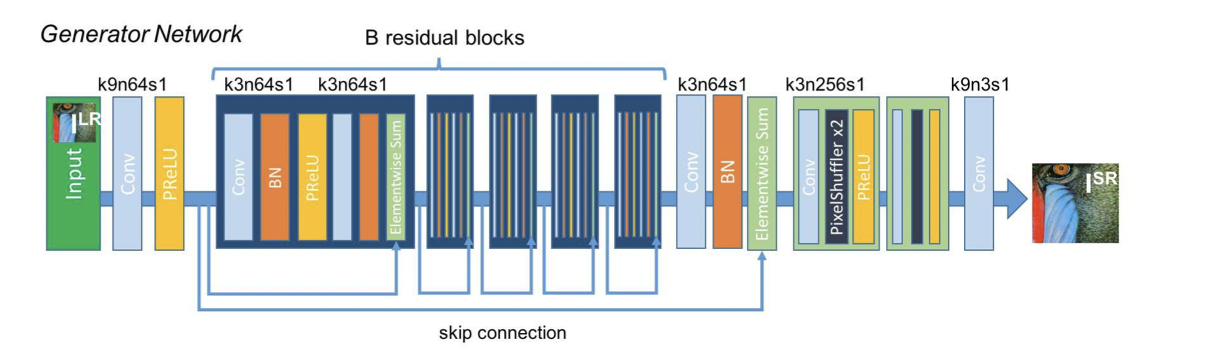
\includegraphics[width=\linewidth]{SRResNet.png}
        \caption{Architecture of the SRResNet}
    \end{subfigure}
\end{figure}

\subsection{Architecture of the Classifier}
The standard architecture of ResNet18 shown in \ref{fig:enter-label} is used.

\subsubsection{Input Layer}
The input to ResNet-18 is typically a 3-channel (RGB) image, and its dimensions depend on the specific task and data set it is designed for.

\subsubsection{Convolutional Layer}
The network starts with a standard convolutional layer with 64 filters, a kernel size of 7x7, and a stride of 2, which reduces the spatial dimensions.

\subsubsection{Batch Normalization and Activation}
After each convolutional layer, batch normalization and a ReLU (Rectified Linear Unit) activation function are applied to introduce non-linearity and improve training stability.

\subsubsection{Residual Blocks}
ResNet-18 consists of four residual blocks, each containing multiple convolutional layers. Each block has the following structure:
\begin{enumerate}
    \item Convolution Layers: Typically, two 3x3 convolutional layers are used in each block.
    \item Batch Normalization and ReLU activation are applied after each convolution.
    \item Shortcut Connection: A ``skip connection" or ``identity shortcut" allows the input to bypass the convolutional layers in the block. This connection helps to mitigate the vanishing gradient problem and facilitates training of very deep networks.
    \item Merge Operation: The output of the convolutional layers is added to the shortcut connection, creating a residual connection. This addition operation is element-wise.
\end{enumerate}

\subsubsection{Down sampling}
After the first residual block, there is a down sampling operation, typically performed by a convolutional layer with a stride of 2. This reduces the spatial dimensions while increasing the number of filters.

\subsubsection{Fully Connected Layer}
The global average pooling operation is applied to the output of the last residual block to reduce the spatial dimensions to a 1x1 feature map. A fully connected layer with the desired number of output neurons is added on top of the global average pooling layer to make predictions for the specific task (e.g., classification).

\subsubsection{Output Layer}
The final layer is typically a softmax activation for classification tasks, providing class probabilities.

\begin{figure}
    \centering
    \begin{subfigure}{0.5\textwidth}
        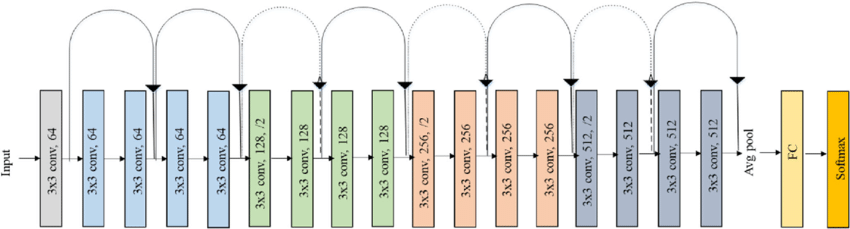
\includegraphics[width=\linewidth]{ResNet18 - 1.png}
    \end{subfigure}
    \caption{Architecture of the CNN}
    \label{fig:enter-label}
\end{figure}

\section{Experiments}
After going through the computation and training of the SRResNet, we realize that the computational complexity to train such a network on new data sets would be beyond the resources available at this time. Hence, we use an off the shelf pre-trained SRResNet for experimenting using the CIFAR-10 and CIFAR-100 data set, as the existing SRResNet was trained on more or less natural images.

Training on this setting has been done without any hyper-parameter tuning. A constant learning rate of 0.001 was used for training the classifier. The classifier was a pre-trained ResNet18. It is further fine-tuned on our data sets. It is observed that the SRResNet architecture performs better than the bicubic interpolation, as shown in table \ref{tab:my_label}.

We have improved on the preliminary results and moved to the domain of medical images. dermaMNIST, pathMNIST, and retinaMNIST data sets have been used to train and test three different architectures, model taking inputs as enlarged images using bicubic interpolation, model taking inputs as enlarged images using SRRestNet, and model taking in unmodified images.

\section{Results and Observations}

\subsection{LR model}
From the training and tuning plots, we observe that performs as well as the other two models initially on the dermaMNIST data set. With respect to the pathMNIST and retinaMNIST data set, the model performs poorly in relation. The accuracy of the LR model does not increase significantly with tuning. The model achieves an accuracy of 73\%, 90\%, and 45\% on dermaMNIST, pathMNIST, retinaMNIST respectively.

\subsection{Bicubic model}
From the training and tuning plots, we observe that the bicubic model performs as good as the SRRestNet. This came as a surprise to the authors, as we expected the SRResNet model to perform better by a higher margin than observed. In the case of retinaMNIST, the bicubic model beats the SRResNet model by 5\%! Tuning the model does improve its performance significantly. The model achieves an accuracy of 77\%, 97\%, and 54\% on dermaMNIST, pathMNIST, retinaMNIST respectively.

\subsection{SRResNet model}
From the training and testing plots, we observe that the SRResNet model achieves accuracies comparable to the bicubic model. Fine tuning the model does help and it hits an accuracy of 77\%, 97\%, and 48\% on dermaMNIST, pathMNIST, retinaMNIST respectively.

We conducted our experiments using the PathMNIST dataset, a medical imaging dataset with nine distinct classes. 
For super-resolution preprocessing, we utilized an off-the-shelf SR Resnet model, pretrained on natural images. Due to the unavailability of high-resolution medical images for training a specific model, this pretrained approach served as a practical solution for enhancing the resolution of our PathMNIST dataset.
The classification model employed in our experiments is a modified version of the ResNet18 architecture. This modification ensures that the model outputs the same number of logits as the classes present in the PathMNIST dataset.
To evaluate the performance of our models, we adhered to the official train-validation-test split provided by the dataset, allocating 90K images for training, 10K for validation, and 7K for testing.
We trained our models for 100 epochs, with a batch size of 64, using the Adam optimizer with a learning rate of 0.001. We used the Cross-Entropy Loss function to train our models.
We evaluated the performance of our models on the test set, reporting the accuracy and loss values. 
All experiments were conducted in a Python 3.10 environment, using PyTorch 2.0 and CUDA 11.1.

\subsection*{Results}
Our experiments revealed that the SRResNet model outperformed the bicubic interpolation approach, achieving an accuracy of 89\% and a loss of 0.32, compared to 88\% accuracy and 0.34 loss for the bicubic interpolation approach. These results indicate that SRResNet can be used to enhance the resolution of medical images, improving the accuracy of classification models.
\begin{table}[h]
    \centering
\section{Future Work}
We are currently working on training the SRResNet on medical image data sets. We are also working on training the classifier on the same data sets, from scratch. We aim to showcase the improvement in accuracy of the classifier when trained on the SRResNet generated images.

\begin{table} 
    \begin{center}
    \begin{tabular}{|| c | c | c ||}
        \hline
        Architecture & Accuracy & Loss \\
        \hline\hline
        Bicubic Interpolation & $0.88$  & $0.34$ \\
        \hline
        SRResNet &  $\mathbf{0.89} $ & $\mathbf{0.32}$ \\
        \hline
    \end{tabular}
    \caption{Comparision of accuracies (in \%) }
    \label{tab:my_label}
\end{table}


\section{Future Work}
% We are currently working on training the SRResNet on medical image datasets. We are also working on training the classifier on the same datasets, from scratch. We aim to showcase the improvement in accuracy of the classifier when trained on the SRResNet generated images. 

% \begin{table} 
%     \begin{center}
%     \begin{tabular}{|| c | c | c ||}
%         \hline
%         Architecture & CIFAR-10 & CIFAR-100 \\
%         \hline\hline
%         Bicubic Interpolation & $93.51$  & $76.04$ \\
%         \hline
%         SRResNet &  $\mathbf{94.15} $ & $\mathbf{77.12}$ \\
%         \hline
%     \end{tabular}
    
%     \caption{Comparision of accuracies (in \%) }
%     \label{tab:my_label}
%     \end{center}
% \end{table}

%%%%%%%%% REFERENCES
{\small
\bibliographystyle{ieee_fullname}
\bibliography{egbib}
}

\end{document}